% NOTE: Sciposter is dependent on the following packages: a0size, boxedminipage, color,
% graphics, ifthen, shadow, times
% You need to have these packages installed for for sciposter to run properly

\documentclass[landscape,26pt]{sciposter}

%%% Document Class Options %%%%
%portrait		% The default, orients paper in portrait mode
%landscape 		% Orients paper in landscape mode		
%boxedsections	% The default, makes section titles appear in boxes
%ruledsections	% Makes section titles appear underlined
%plain sections	% Makes section titles appear plain 


\usepackage{epsfig}
\usepackage{amsmath}
\usepackage{amssymb}
\usepackage{multicol}
\usepackage{wallpaper}
\usepackage{rotating}
\usepackage{verbatim}
\usepackage{epstopdf}

\newtheorem{Def}{Definition}
%\renewcommand{\titlesize}{\Huge}
%\renewcommand{\authorsize}{\Large}
%\renewcommand{\instsize}{\large}
\renewcommand{\sectionsize}{\Large}
\title{ Modular Controllers \\for Jumping Motions}

% The author's or authors' names
\author{\ \\ Ian Ooi and Barbara Cutler}
 
% insert correct institute name
\institute{Department of Computer Science\\
           Rensselaer Polytechnic Institute\\}

\email{ooii@rpi.edu,cutler@cs.rpi.edu}  % shows author email address below institute

\noleftlogo
\norightlogo

%\setlength{\wpXoffset}{-30in}
%\setlength{\wpYoffset}{-32.2in}
%%%%%%%%%%%%%%%%%%%%%%%%%%%%%%%%%%%%%%%%%%%%%%%%%%%%%%%%%%%%%%%%%%%%%%%%%%%%%%%%
\begin{document}
%%%%%%%%%%%%%%%%%%%%%%%%%%%%%%%%%%%%%%%%%%%%%%%%%%%%%%%%%%%%%%%%%%%%%%%%%%%%%%%%


\maketitle

\begin{minipage}[t]{10.5in}
	\section*{Overview}
		We describe composable controllers for the generation of plausible human jumping motions with a forward physics based simulation.  The controller breaks the jump into several steps, consisting of takeoff, in-air, and landing phases.  These steps are formulated as sub-controllers which are composed to produce the final simulation.  Takeoff is broken into a lead-up, windup, and upward thrust, where the character attempts to target its speed and trajectory to reach a target point in air and target landing position.  In the in-air phase, the character positions to avoid obstacles and to prepare for landing.  To land, the character attempts to reduce impact on the joints by minimizing jerk $(\frac{da}{dt})$ in a feet-first landing scheme.

		\vspace{.3in}
	\section*{Goals}
		\begin{itemize}
			\item Development of control algorithm for jumping motion divided into stages 
			\item Demonstration of control algorithm in a variety of situations, showing adaptivity of the system to different heights, distances, and obstacles in between
			\item Deconstruction of the motion into composable segments for a modular approach to the overall motion
		\end{itemize}

		\vspace{.3in}

		\section*{Sketch of the stages of jumping}
			\begin{figure}
				\centering
				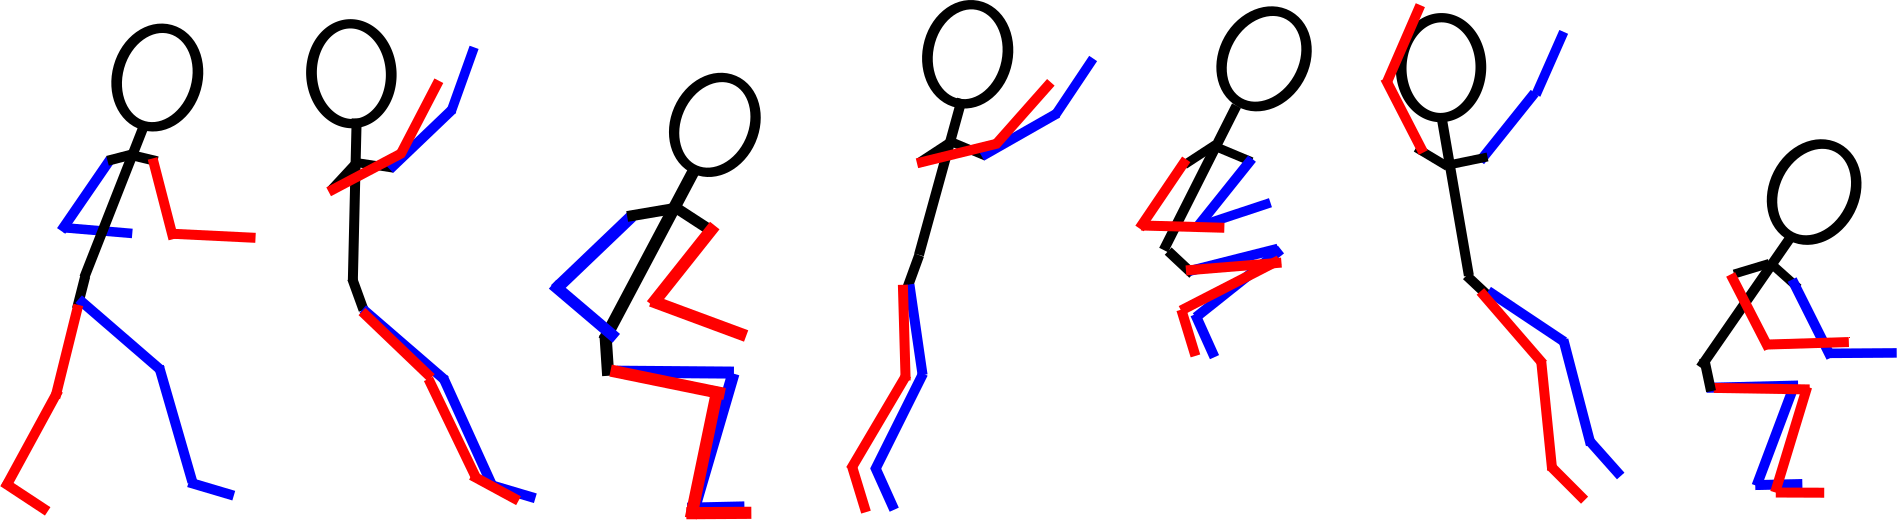
\includegraphics[width=0.8\columnwidth]{movement_sketches/combined_jump.eps}
				\caption{
			We break the motion of jumping into three phases: takeoff, in-	air, and landing.  The focus is on the takeoff, which is itself broken into a lead-up, wind-up, and take off.  The lead-up is a phase in which the character gathers forward momentum, which is partially converted into upward thrust by the wind-up.  The angle at which the character positions its legs ($\theta$) allows it to use the linear velocity to compress the legs and gather spring potential energy, which can be used for an upward thrust.  For in-air, the character re-positions its legs for landing, and finally, in the landing phase, uses the springiness of the legs to maximize the time over which the force is distributed (minimize $\frac{da}{dt}$).}
			\end{figure}
			
	\end{minipage}
	\hfill
\begin{minipage}[t]{17in}
	\section*{Background}
		Producing athletic animations for human characters is difficult.  One method, motion capture is used for production of realistic animations for human athletics and other motions, however it requires the collection of information for each motion and does not adapt to the virtual environment.  Muscle-based approaches produce realistic motions which adapt to the environment, using a complex model of the musculo-skeletal structure.  Geijtenbeek et al. use a rough, user created muscle routing on a skeleton to produce various gaits that are learned based on the velocity and environment.  The muscle routing is optimized to remain within a region while providing optimal forces on the skeleton based on freedom of motion of the skeletal joints and the calculated optimal length of the muscle.  This model is then used to compute sequences of muscle activations, modeling neural signals, which produce the final animations.  This method is effective, producing good results in various levels of gravity on at least 10 different bipedal skeletons \cite{muscle_based_bipeds}.

		\begin{figure}
			\centering
			\includegraphics[width=0.2\columnwidth]{muscle_based/muscle_routing.eps}
			\caption{Example of a muscle routing on a skeleton from Geijtenbeek et al. \cite{muscle_based_bipeds}.}
		\end{figure}
		
		Inverse kinematics approaches attempt to generate the motion based on a desired final position, determining the skeletal position by solving the system given constraints.  Koga et. al use path planning, inverse kinematics, and forward simulation to generate animations of arm motions for robots and humans working cooperatively.  They produce arm manipulations that avoid collisions and result in final positions and orientations for specified parts of the arm to produce motions such as a human putting on glasses and a robot arm and human cooperating to flip a chessboard \cite{motion_intentions}.  
		
		\begin{figure}
			\centering
			\includegraphics[width=0.3\columnwidth]{falling_motion/falling1.eps}
			\hspace{0.1\columnwidth}
			\includegraphics[width=0.3\columnwidth]{falling_motion/falling3.eps}
			\caption{Breakdown of a hands-first falling approach from Ha et al. \cite{falling_landing} and of a feet-first landing approach.  Ha et al. use a rolling strategy to minimize stress on the body and produce a realistic fall.}
		\end{figure}
		
		Physical simulations utilize a rigid-body character with a user-defined skeleton to find optimal poses based on desired conditions.  Ha et al. utilize such a scheme to generate landing motions for human characters based off linear velocity, global angular velocity, and angle of attack.  The system chooses either a feet first or hands first landing strategy and moves into a roll to reduce stress on the body using principles from biomechanics and robotics.  A sampling method is applied to determine successful conditions, producing bounding planes for the data.  The movement is broken into stages of airborne and landing, in which the character re-positions for the designated landing strategy, and executes the landing strategy respectively. Each of these is separated into impact, roll, and get-up stages.  Movement and joint positions are produced using PID servos \cite{falling_landing}.  Other work on producing such controllers was produced by Faloutsos et al. who described a method of composing such controllers by giving pre-conditions, post-conditions, and intermediate state requirements.  The composed controllers are then chosen at each step based on the current pose and which controller is deemed most suitable \cite{composable_controllers}.  Hodgins et al. created several controllers for running, vaulting, and bicycling, creating realistic motions and secondary motion using rigid bodies and spring-mass simulations \cite{anim_human_athletics}.  Geijtenbeek and Pronost provide a detailed review of physics based simulations \cite{inter_physics_anim}.

\end{minipage}
%
\hfill
%%%%%%%%%%%%%%%%%%%%%%%%%%%%%%%%%%%%%%%%%%%%%%%%%%%%%%%%%%%%%%%%%%%%%%%%%%%%%%%%%%%%%%%
\begin{minipage}[t]{14in}
	
	\section*{Future Work}
		To produce realistic animations, we will require an optimizable model of the stages of the jump.  Effective jumping can be broken into several phases: lead-up, take-off, airborne, and landing.  The lead-up phase can be taken as an initial condition providing forward, linear velocity.  Variables to consider include the angle of the legs during the wind-up (called a ``block'' in parkour and freerunning), angle of take-off, linear velocity, and the length and height of the jump.  The jump will be targeted to a particular height at the peak and a landing position.  When jumping, the feet must be repositioned to prepare for a landing, moving from feet behind the character's frontal plane to in front of the frontal plane.  For the airborne phase, the character tucks its legs to avoid collisions, before landing in a similar manner to the feet-first method described in Ha et al. (sans roll) \cite{falling_landing}.
		\vspace{0.3in}
		\begin{figure}
			\centering
			\includegraphics[width=0.5\columnwidth]{falling_motion/falling2.eps}
			\caption{An example of a generated falling motion from Ha et al. \cite{falling_landing}.}		
		\end{figure}
		
	\vspace{0.3in}

	{\small
	\bibliographystyle{abbrv}
	\nocite{muscle_based_bipeds}
	\nocite{anim_human_athletics}
	\nocite{composable_controllers}
	\nocite{soft_contacts}
	\nocite{falling_landing}
	\nocite{vball_footwork_block}
	\nocite{static_block_jumps}
	\nocite{inter_physics_anim}
	\nocite{opt_motion_synth}
	\nocite{motion_intentions}
	\bibliography{refs}
	}
\end{minipage}
%%%%%%%%%%%%%%%%%%%%%%%%%%%%%%%%%%%%%%%%%%%%%%%%%%%%%%%%%%%%%%%%%%%%%%%%%%%%%%%%%%%%%%%
%%%%%%%%%%%%%%%%%%%%%%%%%%%%%%%%%%%%%%%%%%%%%%%%%%%%%%%%%%%%%%%%%%%%%%%%%%%%%%%%%%%%%%%

\end{document}

